\section{Another type of representation, persistent homology}

The problems with the methods above are: 1. Not considering the order/structure of sentences
in a document; 2. having parameter (e.g. k in KNN, estimated distribution in Naive Bayes) to determine which can not be optimal uniformly for
every prediction. For the sentiment prediction, it is fine. So we change our task 
where we actually need to solve these problems.

In this section, we introduce a method for analyzing a text
without parameters. In fact, we consider all
the thresholds ranging from 0 to infinity. Moreover, we want to be able to
find a meaningful correspondence between the computation and
the structure of the text. We use persistent homology.

This is a project report instead of a course note, so the importance
is not on the details of the algorithm but rather the ideas and experiments.
But the algorithm and the theory in themselves are interesting and not
easy to be found clearly on the internet, so for the clearness of the report
we include concisely the necessary
concepts and key algorithms there \ref{theoretical}.

\subsection{Essay grading}

Inherently, persistent homology is useful when it comes to 3d modeling.
But in data analysis in general, it is also useful (e.g.\ analyze the
performance of a basketball team and get an intuitive view of the team structure).

Here we use the persistent homology to analyze discursive essays and grading (specifically the
richness of their argument structures).

Roughly speaking, a better discursive essay should have a
richer writing structure, (a proposition should be discussed
in different angles, the last paragraph echoes to the beginning etc.).
For example,
in Figure~\ref{apple}, on the right, the essay has a statement, and then some arguments,
finally a conclusion.
On the left, each point represents a sentence.
1 - 2 - 3 - 4 are linked by time order, 1 - 4 are linked because they are similar (within a certain range of distance).
This hole means a good argument. There are also filled triangles (2-simplices), those
sentences form clusters, so they are filled instead of forming holes.

\begin{figure}[H]
  \begin{minipage}{0.80\textwidth}
  \tikzset{every picture/.style={line width=0.75pt}} %set default line width to 0.75pt        

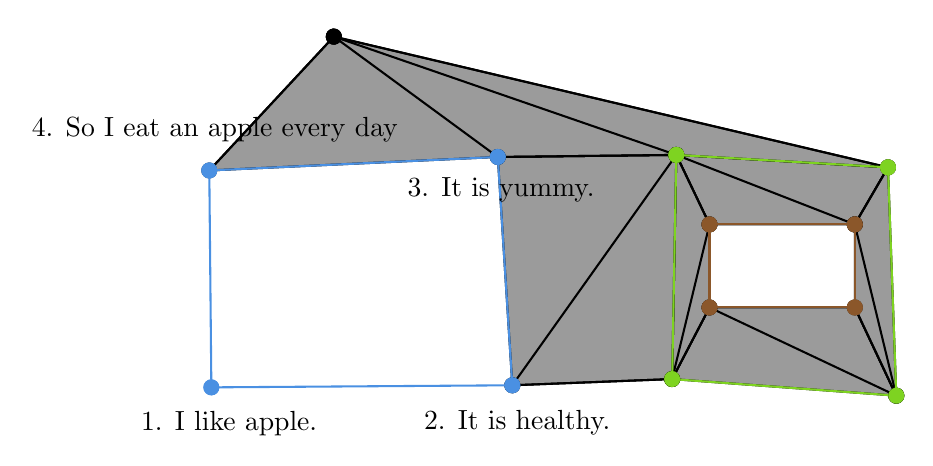
\begin{tikzpicture}[x=0.75pt,y=0.75pt,yscale=-1,xscale=1]
%uncomment if require: \path (0,300); %set diagram left start at 0, and has height of 300

%Shape: Polygon [id:ds506045927728886] 
\draw  [fill={rgb, 255:red, 155; green, 155; blue, 155 }  ,fill opacity=1 ] (337,211.5) -- (355,177) -- (425,177) -- (445,219.5) -- cycle ;
%Shape: Polygon [id:ds373063136182463] 
\draw  [fill={rgb, 255:red, 155; green, 155; blue, 155 }  ,fill opacity=1 ] (441,109.5) -- (425,137) -- (355,137) -- (339,103.5) -- cycle ;
%Shape: Polygon [id:ds04357467087348055] 
\draw  [fill={rgb, 255:red, 155; green, 155; blue, 155 }  ,fill opacity=1 ] (445,219.5) -- (425,177) -- (425,137) -- (441,109.5) -- cycle ;
%Shape: Polygon [id:ds8597694080078087] 
\draw  [fill={rgb, 255:red, 155; green, 155; blue, 155 }  ,fill opacity=1 ] (339,103.5) -- (355,137) -- (355,177) -- (337,211.5) -- cycle ;

%Straight Lines [id:da7958699538877538] 
\draw    (339,103.5) -- (425,137) ;
\draw [shift={(425,137)}, rotate = 21.28] [color={rgb, 255:red, 0; green, 0; blue, 0 }  ][fill={rgb, 255:red, 0; green, 0; blue, 0 }  ][line width=0.75]      (0, 0) circle [x radius= 3.35, y radius= 3.35]   ;
\draw [shift={(339,103.5)}, rotate = 21.28] [color={rgb, 255:red, 0; green, 0; blue, 0 }  ][fill={rgb, 255:red, 0; green, 0; blue, 0 }  ][line width=0.75]      (0, 0) circle [x radius= 3.35, y radius= 3.35]   ;
%Straight Lines [id:da37382810612047734] 
\draw    (425,137) -- (445,219.5) ;
\draw [shift={(445,219.5)}, rotate = 76.37] [color={rgb, 255:red, 0; green, 0; blue, 0 }  ][fill={rgb, 255:red, 0; green, 0; blue, 0 }  ][line width=0.75]      (0, 0) circle [x radius= 3.35, y radius= 3.35]   ;
\draw [shift={(425,137)}, rotate = 76.37] [color={rgb, 255:red, 0; green, 0; blue, 0 }  ][fill={rgb, 255:red, 0; green, 0; blue, 0 }  ][line width=0.75]      (0, 0) circle [x radius= 3.35, y radius= 3.35]   ;
%Straight Lines [id:da33578118329024775] 
\draw    (355,177) -- (445,219.5) ;
\draw [shift={(445,219.5)}, rotate = 25.28] [color={rgb, 255:red, 0; green, 0; blue, 0 }  ][fill={rgb, 255:red, 0; green, 0; blue, 0 }  ][line width=0.75]      (0, 0) circle [x radius= 3.35, y radius= 3.35]   ;
\draw [shift={(355,177)}, rotate = 25.28] [color={rgb, 255:red, 0; green, 0; blue, 0 }  ][fill={rgb, 255:red, 0; green, 0; blue, 0 }  ][line width=0.75]      (0, 0) circle [x radius= 3.35, y radius= 3.35]   ;
%Straight Lines [id:da27555178758587107] 
\draw    (355,137) -- (337,211.5) ;
\draw [shift={(337,211.5)}, rotate = 103.58] [color={rgb, 255:red, 0; green, 0; blue, 0 }  ][fill={rgb, 255:red, 0; green, 0; blue, 0 }  ][line width=0.75]      (0, 0) circle [x radius= 3.35, y radius= 3.35]   ;
\draw [shift={(355,137)}, rotate = 103.58] [color={rgb, 255:red, 0; green, 0; blue, 0 }  ][fill={rgb, 255:red, 0; green, 0; blue, 0 }  ][line width=0.75]      (0, 0) circle [x radius= 3.35, y radius= 3.35]   ;
%Shape: Polygon [id:ds20124875657376728] 
\draw  [fill={rgb, 255:red, 155; green, 155; blue, 155 }  ,fill opacity=1 ] (253,104.5) -- (260,214.5) -- (337,211.5) -- (339,103.5) -- cycle ;
%Shape: Polygon [id:ds3619467537546437] 
\draw  [fill={rgb, 255:red, 155; green, 155; blue, 155 }  ,fill opacity=1 ] (174,46.5) -- (441,109.5) -- (339,103.5) -- (253,104.5) -- (114,111) -- cycle ;
%Straight Lines [id:da5963075508320128] 
\draw    (339,103.5) -- (253,104.5) ;
\draw [shift={(253,104.5)}, rotate = 179.33] [color={rgb, 255:red, 0; green, 0; blue, 0 }  ][fill={rgb, 255:red, 0; green, 0; blue, 0 }  ][line width=0.75]      (0, 0) circle [x radius= 3.35, y radius= 3.35]   ;
\draw [shift={(339,103.5)}, rotate = 179.33] [color={rgb, 255:red, 0; green, 0; blue, 0 }  ][fill={rgb, 255:red, 0; green, 0; blue, 0 }  ][line width=0.75]      (0, 0) circle [x radius= 3.35, y radius= 3.35]   ;
%Straight Lines [id:da8612090103920278] 
\draw    (260,214.5) -- (339,103.5) ;
\draw [shift={(339,103.5)}, rotate = 305.44] [color={rgb, 255:red, 0; green, 0; blue, 0 }  ][fill={rgb, 255:red, 0; green, 0; blue, 0 }  ][line width=0.75]      (0, 0) circle [x radius= 3.35, y radius= 3.35]   ;
\draw [shift={(260,214.5)}, rotate = 305.44] [color={rgb, 255:red, 0; green, 0; blue, 0 }  ][fill={rgb, 255:red, 0; green, 0; blue, 0 }  ][line width=0.75]      (0, 0) circle [x radius= 3.35, y radius= 3.35]   ;
%Straight Lines [id:da9692653745827828] 
\draw    (260,214.5) -- (337,211.5) ;
\draw [shift={(337,211.5)}, rotate = 357.77] [color={rgb, 255:red, 0; green, 0; blue, 0 }  ][fill={rgb, 255:red, 0; green, 0; blue, 0 }  ][line width=0.75]      (0, 0) circle [x radius= 3.35, y radius= 3.35]   ;
\draw [shift={(260,214.5)}, rotate = 357.77] [color={rgb, 255:red, 0; green, 0; blue, 0 }  ][fill={rgb, 255:red, 0; green, 0; blue, 0 }  ][line width=0.75]      (0, 0) circle [x radius= 3.35, y radius= 3.35]   ;
%Straight Lines [id:da7164877740446134] 
\draw    (114,111) -- (174,46.5) ;
\draw [shift={(174,46.5)}, rotate = 312.93] [color={rgb, 255:red, 0; green, 0; blue, 0 }  ][fill={rgb, 255:red, 0; green, 0; blue, 0 }  ][line width=0.75]      (0, 0) circle [x radius= 3.35, y radius= 3.35]   ;
\draw [shift={(114,111)}, rotate = 312.93] [color={rgb, 255:red, 0; green, 0; blue, 0 }  ][fill={rgb, 255:red, 0; green, 0; blue, 0 }  ][line width=0.75]      (0, 0) circle [x radius= 3.35, y radius= 3.35]   ;
%Straight Lines [id:da2125405974487078] 
\draw    (174,46.5) -- (253,104.5) ;
\draw [shift={(253,104.5)}, rotate = 36.29] [color={rgb, 255:red, 0; green, 0; blue, 0 }  ][fill={rgb, 255:red, 0; green, 0; blue, 0 }  ][line width=0.75]      (0, 0) circle [x radius= 3.35, y radius= 3.35]   ;
\draw [shift={(174,46.5)}, rotate = 36.29] [color={rgb, 255:red, 0; green, 0; blue, 0 }  ][fill={rgb, 255:red, 0; green, 0; blue, 0 }  ][line width=0.75]      (0, 0) circle [x radius= 3.35, y radius= 3.35]   ;
%Straight Lines [id:da8884288301278187] 
\draw    (174,46.5) -- (441,109.5) ;
\draw [shift={(441,109.5)}, rotate = 13.28] [color={rgb, 255:red, 0; green, 0; blue, 0 }  ][fill={rgb, 255:red, 0; green, 0; blue, 0 }  ][line width=0.75]      (0, 0) circle [x radius= 3.35, y radius= 3.35]   ;
\draw [shift={(174,46.5)}, rotate = 13.28] [color={rgb, 255:red, 0; green, 0; blue, 0 }  ][fill={rgb, 255:red, 0; green, 0; blue, 0 }  ][line width=0.75]      (0, 0) circle [x radius= 3.35, y radius= 3.35]   ;
%Straight Lines [id:da3878057357434834] 
\draw    (174,46.5) -- (339,103.5) ;
\draw [shift={(339,103.5)}, rotate = 19.06] [color={rgb, 255:red, 0; green, 0; blue, 0 }  ][fill={rgb, 255:red, 0; green, 0; blue, 0 }  ][line width=0.75]      (0, 0) circle [x radius= 3.35, y radius= 3.35]   ;
\draw [shift={(174,46.5)}, rotate = 19.06] [color={rgb, 255:red, 0; green, 0; blue, 0 }  ][fill={rgb, 255:red, 0; green, 0; blue, 0 }  ][line width=0.75]      (0, 0) circle [x radius= 3.35, y radius= 3.35]   ;
%Straight Lines [id:da3895078416872] 
\draw [color={rgb, 255:red, 126; green, 211; blue, 33 }  ,draw opacity=1 ]   (445,219.5) -- (337,211.5) ;
\draw [shift={(337,211.5)}, rotate = 184.24] [color={rgb, 255:red, 126; green, 211; blue, 33 }  ,draw opacity=1 ][fill={rgb, 255:red, 126; green, 211; blue, 33 }  ,fill opacity=1 ][line width=0.75]      (0, 0) circle [x radius= 3.35, y radius= 3.35]   ;
\draw [shift={(445,219.5)}, rotate = 184.24] [color={rgb, 255:red, 126; green, 211; blue, 33 }  ,draw opacity=1 ][fill={rgb, 255:red, 126; green, 211; blue, 33 }  ,fill opacity=1 ][line width=0.75]      (0, 0) circle [x radius= 3.35, y radius= 3.35]   ;
%Straight Lines [id:da300892222460144] 
\draw [color={rgb, 255:red, 74; green, 144; blue, 226 }  ,draw opacity=1 ]   (114,111) -- (115,215.5) ;
\draw [shift={(115,215.5)}, rotate = 89.45] [color={rgb, 255:red, 74; green, 144; blue, 226 }  ,draw opacity=1 ][fill={rgb, 255:red, 74; green, 144; blue, 226 }  ,fill opacity=1 ][line width=0.75]      (0, 0) circle [x radius= 3.35, y radius= 3.35]   ;
\draw [shift={(114,111)}, rotate = 89.45] [color={rgb, 255:red, 74; green, 144; blue, 226 }  ,draw opacity=1 ][fill={rgb, 255:red, 74; green, 144; blue, 226 }  ,fill opacity=1 ][line width=0.75]      (0, 0) circle [x radius= 3.35, y radius= 3.35]   ;
%Straight Lines [id:da5712067967796253] 
\draw [color={rgb, 255:red, 74; green, 144; blue, 226 }  ,draw opacity=1 ]   (115,215.5) -- (260,214.5) ;
\draw [shift={(260,214.5)}, rotate = 359.6] [color={rgb, 255:red, 74; green, 144; blue, 226 }  ,draw opacity=1 ][fill={rgb, 255:red, 74; green, 144; blue, 226 }  ,fill opacity=1 ][line width=0.75]      (0, 0) circle [x radius= 3.35, y radius= 3.35]   ;
\draw [shift={(115,215.5)}, rotate = 359.6] [color={rgb, 255:red, 74; green, 144; blue, 226 }  ,draw opacity=1 ][fill={rgb, 255:red, 74; green, 144; blue, 226 }  ,fill opacity=1 ][line width=0.75]      (0, 0) circle [x radius= 3.35, y radius= 3.35]   ;
%Straight Lines [id:da998130260097339] 
\draw [color={rgb, 255:red, 74; green, 144; blue, 226 }  ,draw opacity=1 ]   (260,214.5) -- (253,104.5) ;
\draw [shift={(253,104.5)}, rotate = 266.36] [color={rgb, 255:red, 74; green, 144; blue, 226 }  ,draw opacity=1 ][fill={rgb, 255:red, 74; green, 144; blue, 226 }  ,fill opacity=1 ][line width=0.75]      (0, 0) circle [x radius= 3.35, y radius= 3.35]   ;
\draw [shift={(260,214.5)}, rotate = 266.36] [color={rgb, 255:red, 74; green, 144; blue, 226 }  ,draw opacity=1 ][fill={rgb, 255:red, 74; green, 144; blue, 226 }  ,fill opacity=1 ][line width=0.75]      (0, 0) circle [x radius= 3.35, y radius= 3.35]   ;
%Straight Lines [id:da15833915226992357] 
\draw [color={rgb, 255:red, 74; green, 144; blue, 226 }  ,draw opacity=1 ]   (114,111) -- (253,104.5) ;
\draw [shift={(253,104.5)}, rotate = 357.32] [color={rgb, 255:red, 74; green, 144; blue, 226 }  ,draw opacity=1 ][fill={rgb, 255:red, 74; green, 144; blue, 226 }  ,fill opacity=1 ][line width=0.75]      (0, 0) circle [x radius= 3.35, y radius= 3.35]   ;
\draw [shift={(114,111)}, rotate = 357.32] [color={rgb, 255:red, 74; green, 144; blue, 226 }  ,draw opacity=1 ][fill={rgb, 255:red, 74; green, 144; blue, 226 }  ,fill opacity=1 ][line width=0.75]      (0, 0) circle [x radius= 3.35, y radius= 3.35]   ;
%Straight Lines [id:da1551244874188762] 
\draw    (441,109.5) -- (425,137) ;
\draw [shift={(425,137)}, rotate = 120.19] [color={rgb, 255:red, 0; green, 0; blue, 0 }  ][fill={rgb, 255:red, 0; green, 0; blue, 0 }  ][line width=0.75]      (0, 0) circle [x radius= 3.35, y radius= 3.35]   ;
\draw [shift={(441,109.5)}, rotate = 120.19] [color={rgb, 255:red, 0; green, 0; blue, 0 }  ][fill={rgb, 255:red, 0; green, 0; blue, 0 }  ][line width=0.75]      (0, 0) circle [x radius= 3.35, y radius= 3.35]   ;
%Straight Lines [id:da45803051915893067] 
\draw    (425,177) -- (445,219.5) ;
\draw [shift={(445,219.5)}, rotate = 64.8] [color={rgb, 255:red, 0; green, 0; blue, 0 }  ][fill={rgb, 255:red, 0; green, 0; blue, 0 }  ][line width=0.75]      (0, 0) circle [x radius= 3.35, y radius= 3.35]   ;
\draw [shift={(425,177)}, rotate = 64.8] [color={rgb, 255:red, 0; green, 0; blue, 0 }  ][fill={rgb, 255:red, 0; green, 0; blue, 0 }  ][line width=0.75]      (0, 0) circle [x radius= 3.35, y radius= 3.35]   ;
%Straight Lines [id:da3656558768012268] 
\draw    (355,177) -- (337,211.5) ;
\draw [shift={(337,211.5)}, rotate = 117.55] [color={rgb, 255:red, 0; green, 0; blue, 0 }  ][fill={rgb, 255:red, 0; green, 0; blue, 0 }  ][line width=0.75]      (0, 0) circle [x radius= 3.35, y radius= 3.35]   ;
\draw [shift={(355,177)}, rotate = 117.55] [color={rgb, 255:red, 0; green, 0; blue, 0 }  ][fill={rgb, 255:red, 0; green, 0; blue, 0 }  ][line width=0.75]      (0, 0) circle [x radius= 3.35, y radius= 3.35]   ;
%Straight Lines [id:da6696032151723832] 
\draw    (355,137) -- (339,103.5) ;
\draw [shift={(339,103.5)}, rotate = 244.47] [color={rgb, 255:red, 0; green, 0; blue, 0 }  ][fill={rgb, 255:red, 0; green, 0; blue, 0 }  ][line width=0.75]      (0, 0) circle [x radius= 3.35, y radius= 3.35]   ;
\draw [shift={(355,137)}, rotate = 244.47] [color={rgb, 255:red, 0; green, 0; blue, 0 }  ][fill={rgb, 255:red, 0; green, 0; blue, 0 }  ][line width=0.75]      (0, 0) circle [x radius= 3.35, y radius= 3.35]   ;
%Straight Lines [id:da9412473128467516] 
\draw [color={rgb, 255:red, 126; green, 211; blue, 33 }  ,draw opacity=1 ]   (337,211.5) -- (339,103.5) ;
\draw [shift={(339,103.5)}, rotate = 271.06] [color={rgb, 255:red, 126; green, 211; blue, 33 }  ,draw opacity=1 ][fill={rgb, 255:red, 126; green, 211; blue, 33 }  ,fill opacity=1 ][line width=0.75]      (0, 0) circle [x radius= 3.35, y radius= 3.35]   ;
\draw [shift={(337,211.5)}, rotate = 271.06] [color={rgb, 255:red, 126; green, 211; blue, 33 }  ,draw opacity=1 ][fill={rgb, 255:red, 126; green, 211; blue, 33 }  ,fill opacity=1 ][line width=0.75]      (0, 0) circle [x radius= 3.35, y radius= 3.35]   ;
%Straight Lines [id:da40626776597378655] 
\draw [color={rgb, 255:red, 126; green, 211; blue, 33 }  ,draw opacity=1 ]   (441,109.5) -- (445,219.5) ;
\draw [shift={(445,219.5)}, rotate = 87.92] [color={rgb, 255:red, 126; green, 211; blue, 33 }  ,draw opacity=1 ][fill={rgb, 255:red, 126; green, 211; blue, 33 }  ,fill opacity=1 ][line width=0.75]      (0, 0) circle [x radius= 3.35, y radius= 3.35]   ;
\draw [shift={(441,109.5)}, rotate = 87.92] [color={rgb, 255:red, 126; green, 211; blue, 33 }  ,draw opacity=1 ][fill={rgb, 255:red, 126; green, 211; blue, 33 }  ,fill opacity=1 ][line width=0.75]      (0, 0) circle [x radius= 3.35, y radius= 3.35]   ;
%Straight Lines [id:da39887955488152826] 
\draw [color={rgb, 255:red, 126; green, 211; blue, 33 }  ,draw opacity=1 ]   (441,109.5) -- (339,103.5) ;
\draw [shift={(339,103.5)}, rotate = 183.37] [color={rgb, 255:red, 126; green, 211; blue, 33 }  ,draw opacity=1 ][fill={rgb, 255:red, 126; green, 211; blue, 33 }  ,fill opacity=1 ][line width=0.75]      (0, 0) circle [x radius= 3.35, y radius= 3.35]   ;
\draw [shift={(441,109.5)}, rotate = 183.37] [color={rgb, 255:red, 126; green, 211; blue, 33 }  ,draw opacity=1 ][fill={rgb, 255:red, 126; green, 211; blue, 33 }  ,fill opacity=1 ][line width=0.75]      (0, 0) circle [x radius= 3.35, y radius= 3.35]   ;
%Straight Lines [id:da42956969917858223] 
\draw [color={rgb, 255:red, 139; green, 87; blue, 42 }  ,draw opacity=1 ]   (425,137) -- (355,137) ;
\draw [shift={(355,137)}, rotate = 180] [color={rgb, 255:red, 139; green, 87; blue, 42 }  ,draw opacity=1 ][fill={rgb, 255:red, 139; green, 87; blue, 42 }  ,fill opacity=1 ][line width=0.75]      (0, 0) circle [x radius= 3.35, y radius= 3.35]   ;
\draw [shift={(425,137)}, rotate = 180] [color={rgb, 255:red, 139; green, 87; blue, 42 }  ,draw opacity=1 ][fill={rgb, 255:red, 139; green, 87; blue, 42 }  ,fill opacity=1 ][line width=0.75]      (0, 0) circle [x radius= 3.35, y radius= 3.35]   ;
%Straight Lines [id:da14852397184426325] 
\draw [color={rgb, 255:red, 139; green, 87; blue, 42 }  ,draw opacity=1 ]   (425,177) -- (425,137) ;
\draw [shift={(425,137)}, rotate = 270] [color={rgb, 255:red, 139; green, 87; blue, 42 }  ,draw opacity=1 ][fill={rgb, 255:red, 139; green, 87; blue, 42 }  ,fill opacity=1 ][line width=0.75]      (0, 0) circle [x radius= 3.35, y radius= 3.35]   ;
\draw [shift={(425,177)}, rotate = 270] [color={rgb, 255:red, 139; green, 87; blue, 42 }  ,draw opacity=1 ][fill={rgb, 255:red, 139; green, 87; blue, 42 }  ,fill opacity=1 ][line width=0.75]      (0, 0) circle [x radius= 3.35, y radius= 3.35]   ;
%Straight Lines [id:da7173822720349425] 
\draw [color={rgb, 255:red, 139; green, 87; blue, 42 }  ,draw opacity=1 ]   (355,177) -- (425,177) ;
\draw [shift={(425,177)}, rotate = 0] [color={rgb, 255:red, 139; green, 87; blue, 42 }  ,draw opacity=1 ][fill={rgb, 255:red, 139; green, 87; blue, 42 }  ,fill opacity=1 ][line width=0.75]      (0, 0) circle [x radius= 3.35, y radius= 3.35]   ;
\draw [shift={(355,177)}, rotate = 0] [color={rgb, 255:red, 139; green, 87; blue, 42 }  ,draw opacity=1 ][fill={rgb, 255:red, 139; green, 87; blue, 42 }  ,fill opacity=1 ][line width=0.75]      (0, 0) circle [x radius= 3.35, y radius= 3.35]   ;
%Straight Lines [id:da6148683084406998] 
\draw [color={rgb, 255:red, 139; green, 87; blue, 42 }  ,draw opacity=1 ]   (355,177) -- (355,137) ;
\draw [shift={(355,137)}, rotate = 270] [color={rgb, 255:red, 139; green, 87; blue, 42 }  ,draw opacity=1 ][fill={rgb, 255:red, 139; green, 87; blue, 42 }  ,fill opacity=1 ][line width=0.75]      (0, 0) circle [x radius= 3.35, y radius= 3.35]   ;
\draw [shift={(355,177)}, rotate = 270] [color={rgb, 255:red, 139; green, 87; blue, 42 }  ,draw opacity=1 ][fill={rgb, 255:red, 139; green, 87; blue, 42 }  ,fill opacity=1 ][line width=0.75]      (0, 0) circle [x radius= 3.35, y radius= 3.35]   ;

% Text Node
\draw (79.67,225.67) node [anchor=north west][inner sep=0.75pt]   [align=left] {1. I like apple.};
% Text Node
\draw (216,225) node [anchor=north west][inner sep=0.75pt]   [align=left] {2. It is healthy.};
% Text Node
\draw (208,113) node [anchor=north west][inner sep=0.75pt]   [align=left] {3. It is yummy.};
% Text Node
\draw (27,84) node [anchor=north west][inner sep=0.75pt]   [align=left] {4. So I eat an apple every day};


\end{tikzpicture}
  \end{minipage}
  \begin{minipage}{0.19\textwidth}
  $\cdots$I like apple. It is healthy. It is yummy. So I eat an apple every day.
  $\cdots$
  \end{minipage}
  \caption{There are 2 holes in this simplicial complex,
  one represented by the blue cycle and one by brown.
  Note that the brown cycle and the green cycle are homology equivalent, so they count as one.}
  \label{apple}
\end{figure}

If we only have one such graph, we will have to determine the similarity threshold to link.
However, different thresholds can give different insights. Structure changes with scale, e.g.\ Figure~\ref{fig:scale}.
So our approach will consider all the scales (whence ``persistent'' homology).

\begin{figure}[H]
\centering
\includegraphics[width=14cm]{scale.png}
\caption{Structure changes with scale}
\label{fig:scale}
\end{figure}

\begin{figure}[H]
\centering
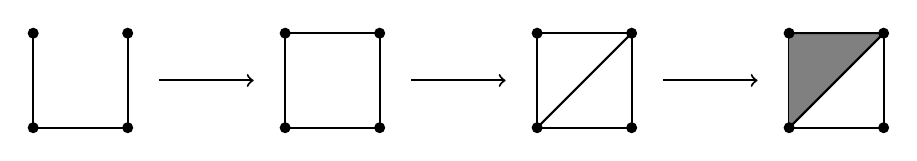
\begin{tikzpicture}[scale=0.4]

  \coordinate (v1) at (0,0);
  \coordinate (v2) at (0,3);
  \coordinate (v3) at (3,0);
  \coordinate (v4) at (3,3);
  \draw (v1) -- (v2);
  \draw (v3) -- (v4);
  \draw (v1) -- (v3);

  \coordinate (w1) at (8+0,0);
  \coordinate (w2) at (8+0,3);
  \coordinate (w3) at (8+3,0);
  \coordinate (w4) at (8+3,3);
  \draw (w1) -- (w2);
  \draw (w3) -- (w4);
  \draw (w1) -- (w3);
  \draw (w2) -- (w4);
  \draw[->] (4,1.5) -- (7,1.5);

  \coordinate (u1) at (16+0,0);
  \coordinate (u2) at (16+0,3);
  \coordinate (u3) at (16+3,0);
  \coordinate (u4) at (16+3,3);
  \draw (u1) -- (u2);
  \draw (u3) -- (u4);
  \draw (u1) -- (u3);
  \draw (u2) -- (u4);
  \draw (u1) -- (u4);
  \draw[->] (12,1.5) -- (15,1.5);

  \coordinate (uu1) at (24+0,0);
  \coordinate (uu2) at (24+0,3);
  \coordinate (uu3) at (24+3,0);
  \coordinate (uu4) at (24+3,3);
  \draw (uu1) -- (uu2);
  \draw (uu3) -- (uu4);
  \draw (uu1) -- (uu3);
  \draw (uu2) -- (uu4);
  \draw (uu1) -- (uu4);
  \filldraw[fill=gray] (uu1) -- (uu4) -- (uu2);
  \draw[->] (20,1.5) -- (23,1.5);

  \foreach \vertex in {v1,v2,v3,v4,w1,w2,w3,w4,
  u1,u2,u3,u4,
  uu1,uu2,uu3,uu4}
    \fill (\vertex) circle (5pt);
\end{tikzpicture}
\caption{We continue linking and filling (e.g.\ triangles) when the $d$ increases; note that
we may have multiple linkings and fillings to do within a same $d$ but we discretize these
for the algorithm}
\label{filtration}
\end{figure}

The algorithm is the following (for the exact version \ref{sifts}) :

We vary $d$ from $0$ to $1$, for every $d$ we create a graph like Figure~\ref{apple}
(points representing sentences are linked first in order in the essay,
then we link sentences whose differences are lower than $d$,
we fill triangles, tetrahedrons, etc. as shown in Figure~\ref{filtration}) What we will get is
$(V_d)_{0\le d\le 1}$, a filtration of graphes one included in another while $d$ increases.
Then there are holes that appear and disappear, we count the number of total appearances of holes.

We hope to show that this number of holes reflects the quality of arguments of an essay.

\paragraph{Experiment on a real set of data}

data source (more precisely, the essay set 2, which is discoursive) :
\url{https://www.kaggle.com/datasets/thevirusx3/automated-essay-scoring-dataset/code?select=training_set_rel3.tsv}

\begin{figure}[H]
\begin{minipage}{0.49\linewidth}
\includegraphics[width=8cm]{pdessay.png}
\end{minipage}
\begin{minipage}{0.49\linewidth}
\begin{mdframed}
In @DATE1's world, there are many things found offensive.  Everyone has their own opinion on what is offensive and what is not. Many parents are becoming upset because they think their children are viewing things that they should not.  Other people are upset because they think the libraries are offending their culture or way of life.  This is even taken to the extreme where people want censhorship on libraries to avoid this, which is wrong.     Some people are becoming concerned about the materials in libraries...($\sim$450 words)
\end{mdframed}
\end{minipage}
\caption{The persistence diagram of an essay of grade 4/6 : A blue point $(x, y)$ in this diagram means
that there is a hole appears at $d=x$ and disappears at $d=y$.
One red point means there is only one connected component the whole time,
because we link all the sentences by order in the essay.
}
\label{fig:pd}
\end{figure}

\begin{figure}[H]
% \centering
\includegraphics[width=8cm]{gradesh1.png}
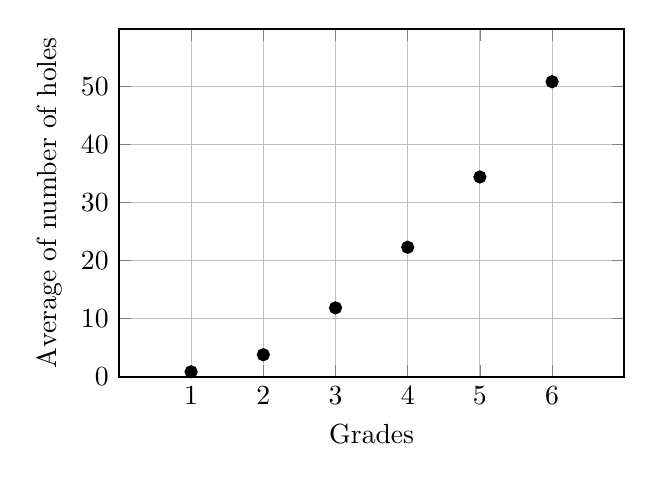
\begin{tikzpicture}
  \begin{axis}[
    xlabel={Grades},
    ylabel={Average of number of holes},
    grid=both,
    xmin=0,
    ymin=0,
    xmax=7,
    ymax=60,
    xtick={1,2,3,4,5,6},
    ytick={0,10,20,30,40,50},
    width=8cm,
    height=6cm,
    ]
    
    \addplot[only marks, mark=*, mark size=2pt] coordinates {
        (1, 0.8333333333333334)
        (2, 3.7777777777777777)
        (3, 11.857142857142858)
        (4, 22.308483290488432)
        (5, 34.42666666666667)
        (6, 50.857142857142854)
    };
  \end{axis}
\end{tikzpicture}
\caption{Number of holes increases as grade increases}
\label{fig:ds}
\end{figure}

Those are some discursive essays on the topic of offense/censorship graded 1-6. We first inspect
an essay with a grade 4/6 as an example Figure~\ref{fig:pd}. Then we show
the average number of holes for each grade (1-6)
as well as the average number of holes for each grade (Figure~\ref{fig:ds}).
We find that number of holes increases as the grade increases.

But there are other factors other than the richness of structure of the essay that may affect
the number of holes, like the number of sentences (if we have more points in the set
we will have more chances to form holes) or the number of words.

\begin{figure}[H]
  \includegraphics[width=8cm]{gradesah1s.png}
  \includegraphics[width=8cm]{gradesah1w.png}
  \caption{The average of holes each sentence/word increases as grade increases (from 1 to 6, upper to lower histogram)}
  \label{fig:ads}
\end{figure}

First, let's try to eliminate the effect of number of sentences/number of words
by dividing it (Figure~\ref{fig:ads}). So as we expected, it still shows a simultaneous
increase in the number of holes and grades. But even now we may suspect that
maybe the number of holes is just the number of sentences squared. To show that
this is not the case, we fix the number of sentences/the number of words in a range
and inspect the number of holes.

\begin{figure}{h}
  \begin{minipage}[t]{0.33\textwidth}
  \centering
  \begin{tabular}{|c|p{2.5cm}|}
  \hline
  \multicolumn{2}{|c|}{Number of Sentences 30-35} \\
  \hline
  Grade & Average of Number of Barcodes \\
  \hline
  3 & 30.75 \\
  4 & 32.0 \\
  5 & 33.06 \\
  6 & 28.33 \\
  \hline
  \end{tabular}
  \end{minipage}%
  \begin{minipage}[t]{0.33\textwidth}
  \centering
  \begin{tabular}{|c|p{2.5cm}|}
  \hline
  \multicolumn{2}{|c|}{Number of Sentences 40-45} \\
  \hline
  Grade & Average of Number of Barcodes \\
  \hline
  3 & 40.0 \\
  4 & 45.96 \\
  5 & 49.45 \\
  6 & 52.0 \\
  \hline
  \end{tabular}
  \end{minipage}%
  \begin{minipage}[t]{0.33\textwidth}
  \centering
  \begin{tabular}{|c|p{2.5cm}|}
  \hline
  \multicolumn{2}{|c|}{Number of Sentences 50-55} \\
  \hline
  Grade & Average of Number of Barcodes \\
  \hline
  3 & 63.0 \\
  4 & 50.0 \\
  5 & 79.0 \\
  \hline
  \end{tabular}
  \end{minipage}

  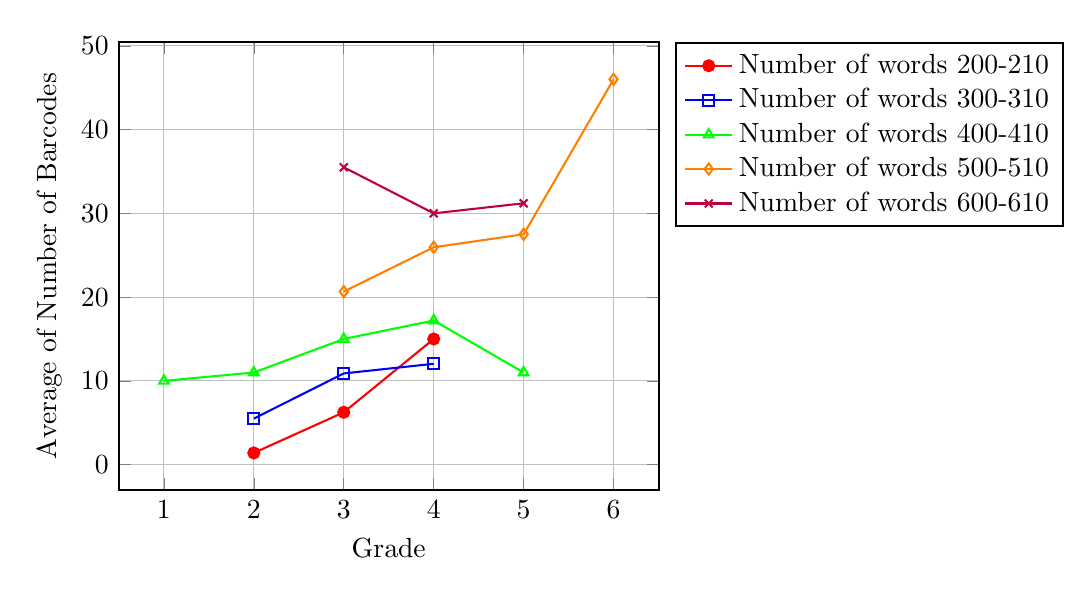
\begin{tikzpicture}
    \begin{axis}[
      xlabel={Grade},
      ylabel={Average of Number of Barcodes},
      legend pos=outer north east,
      grid=both,
    ]
    
    % Number of words 200-210
    \addplot[color=red,mark=*] coordinates {
      (2, 1.4)
      (3, 6.25)
      (4, 15.0)
    };
    
    % Number of words 300-310
    \addplot[color=blue,mark=square] coordinates {
      (2, 5.5)
      (3, 10.89)
      (4, 12.04)
    };
    
    % Number of words 400-410
    \addplot[color=green,mark=triangle] coordinates {
      (1, 10.0)
      (2, 11.0)
      (3, 15.0)
      (4, 17.21)
      (5, 11.0)
    };
    
    % Number of words 500-510
    \addplot[color=orange,mark=diamond] coordinates {
      (3, 20.66)
      (4, 25.95)
      (5, 27.5)
      (6, 46.0)
    };
    
    % Number of words 600-610
    \addplot[color=purple,mark=x] coordinates {
      (3, 35.5)
      (4, 30.0)
      (5, 31.2)
    };
    
    \legend{
      Number of words 200-210,
      Number of words 300-310,
      Number of words 400-410,
      Number of words 500-510,
      Number of words 600-610
    }
    
    \end{axis}
    \end{tikzpicture}

  \caption{Grades and averages of number of holes within fixed sentence/word number ranges}
  \label{tab:gar}
\end{figure}

Seeing Figure~\ref{tab:gar}, we indeed observe and confirm the correlation of increase
that we conjectured. However, the correlation is not absolute as we can constate.
This is because we don't have enough data (for almost all contradictory data
we have selected only one essay of that grade in that range) and other factors than the argument
do affect the grade too (holes only show the structure of an essay, for which we
chose to do the tests on discursive essays). Typically, the wording
of essays of grade 3 but with 30-40 holes is bad and repetitive, which is
probably the reason why they are graded not high.

In conclusion, while in Figure~\ref{fig:ads} we have enough essays as examples with the default that
the method(division) is not rigorously convincing, and in Figure~\ref{tab:gar} we don't
have enough essays for each range though the method is solid, with them combined,
we are confident that the number of holes of dim 1 is a good measure of the quality of
argument structure of an essay. While we changed our task for applying
this topological representation of text, this task can not be achieved by
KNN or Naive Bayes either, because they would both totally ignore
the structure of an essay.

\paragraph{Further} We may provision studying the identification of the type
of arguments (or in the previous case, type of comments) by exploiting persistent homology structure,
trying higher dimensional persistent homology, etc. But our journey ends here.